\documentclass[shrink, compress, mathserif, 10pt, xcolor=dvipsnames,
               aspectratio=169]{beamer}
\usetheme{Scale}

\usepackage{textcomp}
%%\usepackage[french]{babel}
\usepackage[T1]{fontenc}
\usepackage[utf8]{inputenc}
\usepackage{helvet}

\title{Bibliothèque NSIMD}
\subtitle{Application à EFISPEC3D, le prédiction numérique des sismogrammes
          pour le risque sismique}
\date{\today}
\author{Agenium Scale}

\begin{document}

\begin{frame}[plain]
  \maketitle
\end{frame}

\input{NSIMD-fr.tex}

\begin{frame}{Application à EFISPEC3D}
  \begin{itemize}
    \item Prédiction numérique des sismogrammes pour le risque sismique.
    \vspace{1em}
    \item Similaire à SPECFEM3D, extracted from EFISPEC3D developed at BRGM
          (le service géologique national français).
    \vspace{1em}
    \item Le maillage utilisé a pour conséquence que les éléments partagent
          des points sur leurs frontières avec leurs voisins
          $\longrightarrow$ tableaux d'indirections pour éviter de stocker
          des ponits de multiples fois.
    \vspace{1em}
    \item Code original écrit en Fortran.
    \vspace{1em}
    \item Pas de vectorisation automatique (même en utilisant des pragmas) sur
          toutes lesarchitectures/compilateurs.
    \vspace{1em}
    \item Vectorisation doit être faites en utilisant NSIMD.
  \end{itemize}
\end{frame}

\begin{frame}{Temps d'exécution}
  \begin{center}
    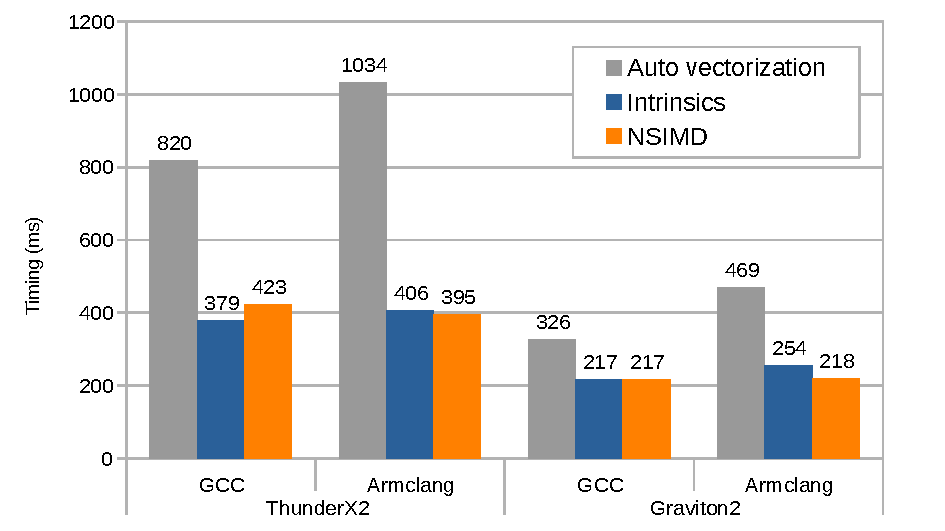
\includegraphics[width=0.55\textwidth]{timings.pdf}
  \end{center}
\end{frame}

\begin{frame}{Conclusion et liens}
  \begin{itemize}
    \item
      Un seul code source pour toutes les extensions SIMD.
    \item
      NSIMD n'a pas d'overhead pour les codes de calcul scientiques et
      industriels.
    \item
      Augmentation de la lisibilité et de la maintenabilité du code.  
  \end{itemize}

  \vspace{2em}
  \begin{enumerate}
    \item EFISPEC3D: \url{https://www.brgm.fr/projet/efispec3d-prediction-numerique-sismogrammes-risque-sismique}
    \item NSIMD: \url{https://github.com/agenium-scale/nsimd}
    \item EFISPEC3D with NSIMD: \url{https://github.com/agenium-scale/EFISPEC3D}
    \item AGENIUM SCALE: \url{https://www.agenium-scale.com}
  \end{enumerate}
\end{frame}

\end{document}
